\subsection{Selección de Ventana}
\label{sec:window_selection}

Otro parámetro de la técnica es el tamaño y step de la ventana, que discutiremos en esta sección. En el trabajo \cite{KOU2008.2} se menciona una elección de \emph{frame step} y \emph{frame length} de 10s y 20s respectivamente. En el caso de nuestro corpus, queremos buscar los parámetros que mejor se ajustan a éste, manteniendo la superposición del 50\% entre ventanas sucesivas.

¿Qué queremos optimizar? La métrica que elegimos para ésto es encontrar un balance entre una ventana no tan grande (para no suavizar en exceso la curva) y que nos reduzca considerablemente la cantidad de indefiniciones; es decir, aquellas ventanas que tomamos en un interlocutor que no tienen ninguna interacción de su parte. Para ver ésto, graficamos la cantidad de indefiniciones en función del step tomado, para ver qué forma tenían estas curvas.

\begin{figure}
\centering
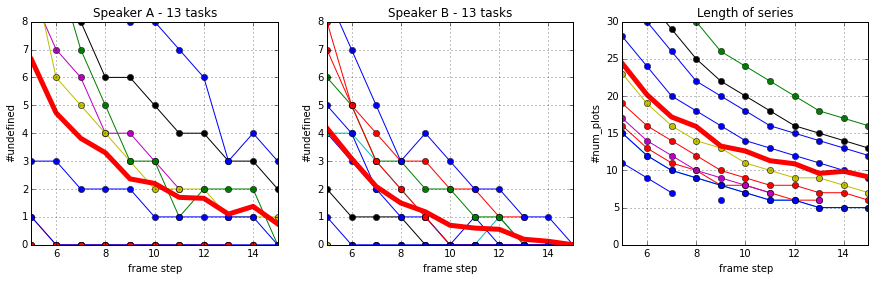
\includegraphics[width=15cm]{images/window_selection_for_session.png}
\caption{Cantidad de puntos indefinidos en función del step para una sesión en particular, tanto para un interlocutor como para el otro. En rojo se grafica la curva de los promedios. }
\end{figure}



Dentro del rango de $FS \in \{5'',6'', \ldots ,15'' \}$, graficamos para cada sesión, tarea y cada interlocutor las curvas de indefiniciones. A su vez, para mayor claridad, graficamos una curva que promedie todas las tareas de una sesión.


Para tener una visión general de lo que ocurría en todas las sesiones, graficamos una curva promedio de todas las sesiones. En ésta puede observarse que hasta $8''-10''$ hay un fuerte descenso de las indefiniciones, que luego se atenúa. Dado que en general tenemos tareas cortas, preferimos tomar $8''$ como step, y $16''$ como largo de ventana.

OBS: podríamos cambiar ésto a un boxplot!

\begin{figure}
\centering
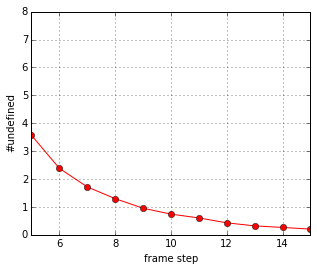
\includegraphics[width=15cm]{images/window_selection.png}
\end{figure}


